\subsubsection*{Count map and distribution}

First step to check whether data that have in our hand is makes some sense or not is to simply plot the distribution of photon from a picked single weekly photon file 
as in Fig \ref{fig:exphotondist}. Another step is to see the histogram of photon over energy as \ref{fig:photoncounthist}.

\begin{figure}
    \centering
    \begin{minipage}[b]{0.49\textwidth}
        \centering
        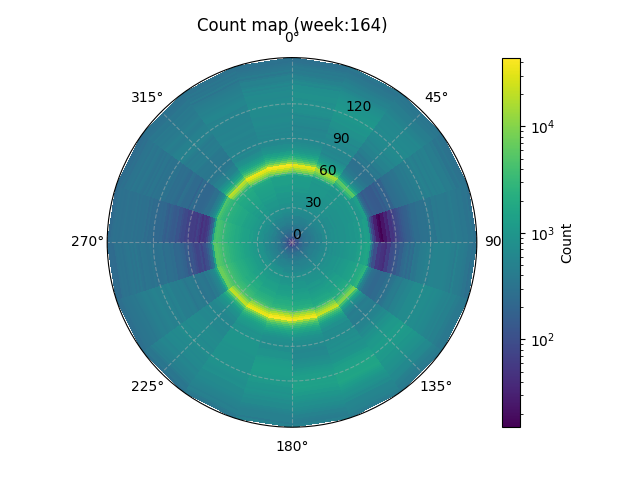
\includegraphics[width=\textwidth]{img/cntmap_polar}
    \end{minipage}
    \begin{minipage}[b]{0.49\textwidth}
        \centering
        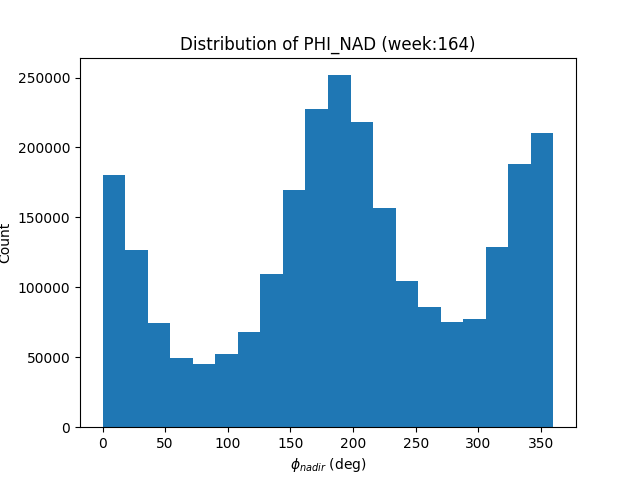
\includegraphics[width=\textwidth]{img/phi_nad_dist}
    \end{minipage}
    \caption{An example distribution of $\gamma$-ray from a single week}
    \label{fig:exphotondist}
\end{figure}


\begin{figure}[h!]
    \centering
    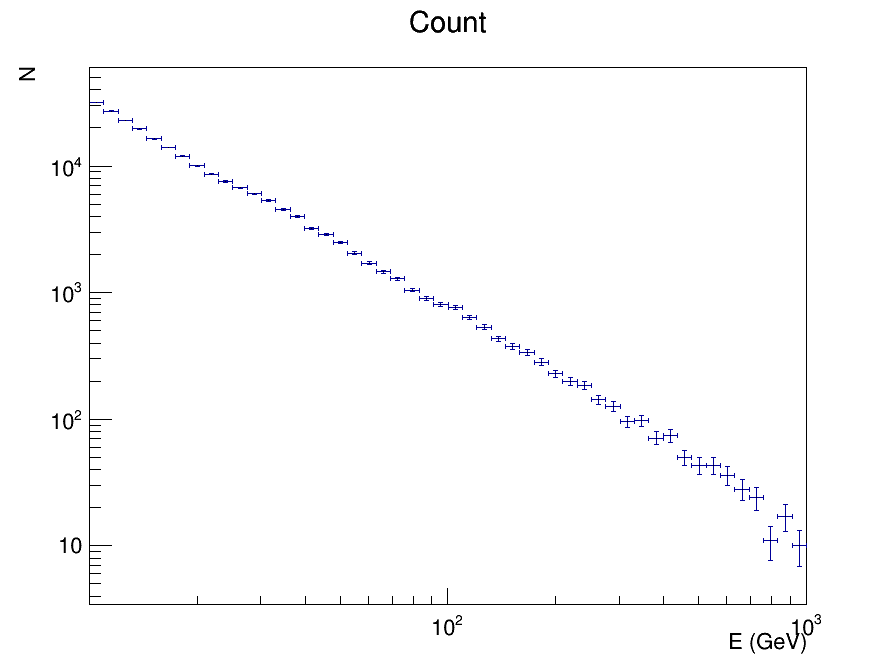
\includegraphics[width=0.8\textwidth]{img/count_hist}
    \caption{Raw histogram of photon in energy}
    \label{fig:photoncounthist}
\end{figure}

\subsubsection*{Exposure maps}

This step require a lot of effort to make it robust and many of testing has been performed from
the serial to parallel code along the way of development.
To overview some of the exposure map, the selected four out of fifty exposure map has shown in the Fig (\ref{fig:expmapscart}, \ref{fig:expmapspolar}) in cartesian and polar plot sequentially.

\begin{figure}[h!]
    \centering
    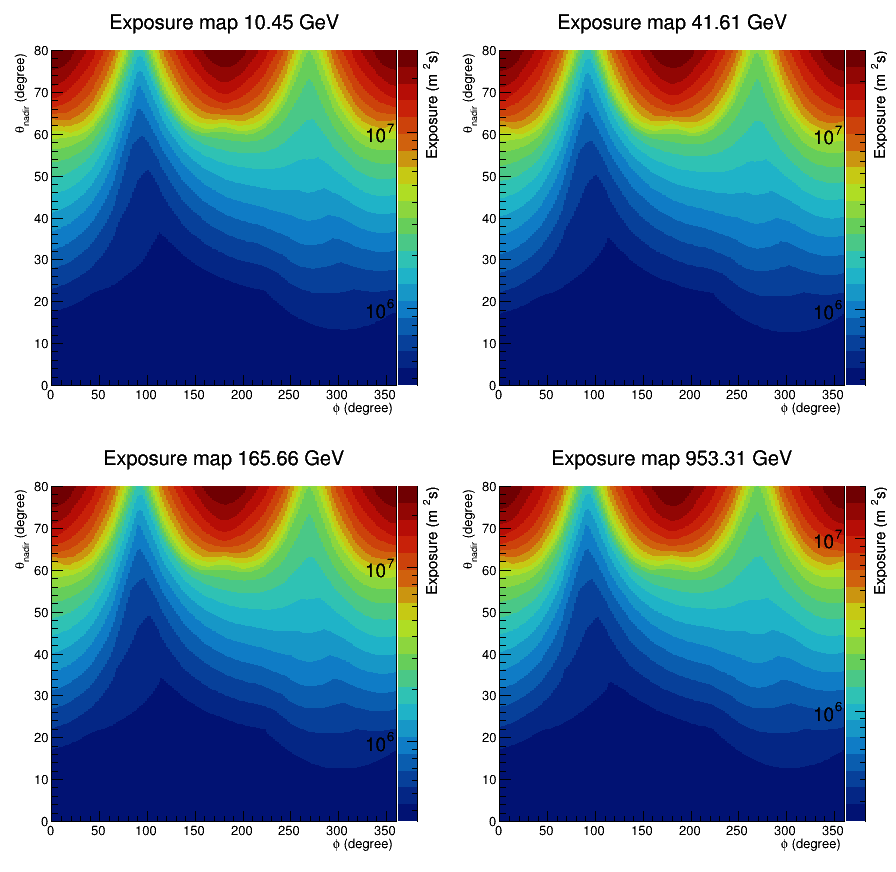
\includegraphics[width=\textwidth]{img/cartesian_expmaps}
    \caption{Exposure map of various $\gamma$-ray energy in cartesian plot}
    \label{fig:expmapscart}
\end{figure}

\begin{figure}[h!]
    \centering
    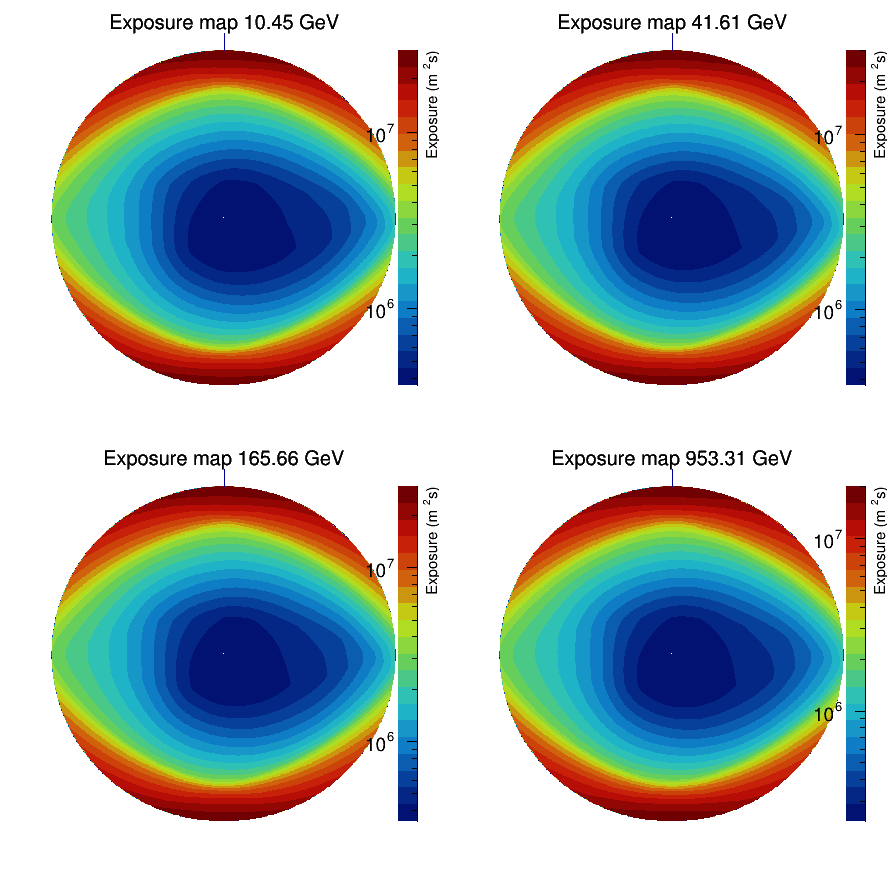
\includegraphics[width=\textwidth]{img/polar_expmaps}
    \caption{Exposure map of various $\gamma$-ray energy in polar plot}
    \label{fig:expmapspolar}
\end{figure}

\subsubsection*{Differential Flux of $\gamma$-ray}

Lastly, preliminary of gamma-ray spectrum has been computed and show in Fig \ref{fig:gammarayfluxnew}.

\begin{figure}[h!]
    \centering
    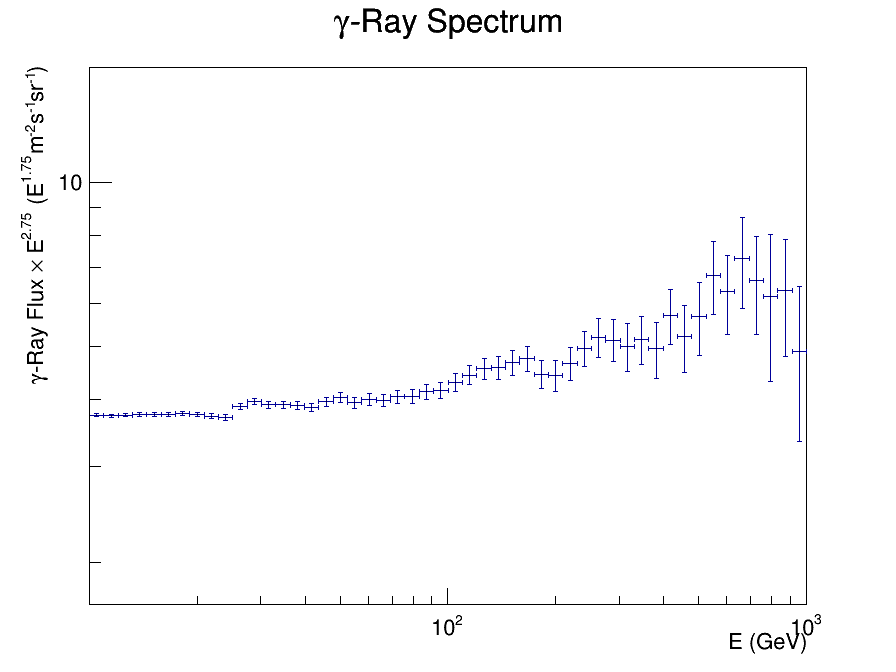
\includegraphics[width=0.8\textwidth]{img/flx_hist_2}
    \caption{$\gamma$-ray spectrum in energy}
    \label{fig:gammarayfluxnew}
\end{figure}

